% B.Tech. Project Report (Phase I) - ECG ring
% Compiles with IEEEtran (Overleaf has it). Without IEEEtran.cls it falls back to
% a two-column article so the draft can still be built anywhere.
\IfFileExists{IEEEtran.cls}{%
  \documentclass[conference,10pt]{IEEEtran}\def\ieeemode{1}}{%
  \documentclass[10pt,twocolumn]{article}\def\ieeemode{0}}

\usepackage[utf8]{inputenc}
\usepackage[T1]{fontenc}
\usepackage{mathptmx}
\usepackage{amsmath,amssymb}
\usepackage{graphicx}
\usepackage{booktabs}
\usepackage{multirow}
\usepackage{xcolor}
\definecolor{navy}{RGB}{31,56,100}
\usepackage{tikz}
\usetikzlibrary{arrows.meta,positioning,fit}
\usepackage{subcaption}
\usepackage{cite}
\usepackage{url}
\usepackage{siunitx}
\sisetup{detect-all}

\if0\ieeemode
  \usepackage[margin=0.75in,columnsep=0.25in]{geometry}
  \newenvironment{IEEEkeywords}{\par\noindent\textbf{\textit{Index Terms}---}}{\par}
  \renewcommand{\abstractname}{}
  \usepackage{titlesec}
  \titleformat{\section}{\centering\normalfont\scshape}{\Roman{section}.}{0.5em}{}
  \titleformat{\subsection}{\normalfont\itshape}{\Alph{subsection}.}{0.5em}{}
\fi

% ---------- placeholders: replace before submission ----------
\newcommand{\TODO}[1]{\textcolor{red}{[#1]}}
\newcommand{\StudentNames}{Dhruva Sharma}
\newcommand{\EnrolmentNos}{23123016}
\newcommand{\Supervisor}{Prof. Bishnu Prasad Das}
\newcommand{\ProjectTitle}{A Finger-Electrode ECG Ring: Validated Acquisition, Beat Timing and Physiological Analytics on a Wearable Platform}

\begin{document}

% =================== Title page and certificate ===================
\onecolumn
\thispagestyle{empty}
\begin{center}
\vspace*{0.5cm}
{\large B.Tech. Project Report (Phase I)}\\[0.6em]
{\color{navy}\rule{0.55\textwidth}{0.8pt}}\\[2.2em]
{\LARGE\bfseries\color{navy} A Finger-Electrode ECG Ring:\\[0.25em] Validated Acquisition, Beat Timing and\\[0.25em] Physiological Analytics on a Wearable Platform\par}
\vspace{2.2em}
{\color{navy}\rule{0.55\textwidth}{0.8pt}}\\[2.4em]
Submitted in partial fulfilment of the requirements for the degree of\\[0.5em]
{\bfseries Bachelor of Technology}\\[0.2em] in\\[0.2em] {\bfseries Electronics and Communication Engineering}\\[3em]
by\\[0.5em]
{\Large\bfseries \StudentNames}\\[0.3em]
Enrolment No. \EnrolmentNos\\[2.6em]
Under the supervision of\\[0.5em]
{\Large\bfseries \Supervisor}\\[3em]

\includegraphics[height=2.6cm]{figs/logo_iitr.png}\hspace{1.6cm}
\includegraphics[height=2.6cm]{figs/logo_ece.png}\\[2.6em]
{\bfseries Department of Electronics and Communication Engineering}\\[0.2em]
{\bfseries Indian Institute of Technology Roorkee}\\[0.2em]
Roorkee -- 247667, Uttarakhand, India\\[0.8em]
Academic Year 2026--27 (Autumn Semester)
\end{center}
\newpage
\thispagestyle{empty}
\begin{center}
\vspace*{0.5cm}

\includegraphics[height=2.2cm]{figs/logo_iitr.png}\\[1em]
{\bfseries Department of Electronics and Communication Engineering}\\[0.2em]
{\bfseries Indian Institute of Technology Roorkee}\\[3em]
{\LARGE\bfseries\color{navy} CERTIFICATE}\\[0.4em]
{\color{navy}\rule{0.25\textwidth}{0.8pt}}
\end{center}
\vspace{2em}
\noindent This is to certify that the project report entitled \textbf{``\ProjectTitle''}, submitted by \textbf{\StudentNames{} (Enrolment No.~\EnrolmentNos)} in partial fulfilment of the requirements for the award of the degree of Bachelor of Technology in Electronics and Communication Engineering, is a record of the work carried out by the candidate under my supervision during the Autumn Semester of the academic year 2026--27, as Phase~I of the B.Tech. project.

\medskip\noindent The work presented in this report has been reviewed and approved for submission.

\vspace{6em}
\noindent
\begin{minipage}[t]{0.45\textwidth}
Date: \rule{3.5cm}{0.4pt}\\[1.2em]
Place: Roorkee
\end{minipage}\hfill
\begin{minipage}[t]{0.42\textwidth}\raggedleft
\rule{5.5cm}{0.4pt}\\[0.3em]
\textbf{\Supervisor}\\
Project Supervisor\\
Department of Electronics and\\ Communication Engineering\\
IIT Roorkee
\end{minipage}
\newpage
\twocolumn

% =================== Paper body ===================
\title{\ProjectTitle}
\if1\ieeemode
\author{\IEEEauthorblockN{\StudentNames}
\IEEEauthorblockA{B.Tech. Project, Phase I $\cdot$ Guide: \Supervisor\\
Department of Electronics and Communication Engineering, Indian Institute of Technology Roorkee}}
\else
\author{\StudentNames\\ \small B.Tech. Project, Phase I $\cdot$ Guide: \Supervisor\\ \small Department of ECE, Indian Institute of Technology Roorkee}
\date{}
\fi
\maketitle

\begin{abstract}
Single-lead ECG recorded between two fingers is the basis of ring and smartphone heart monitors, but small, noisy finger signals and real-time processing on a phone make beat-to-beat measurements fragile. This project builds an ECG acquisition and analysis system around the MAX30003 analogue front end, an ESP32 microcontroller and an Android application, as the platform for a finger-electrode ECG ring. Identical firmware runs on a ring-format board and on a reference board, so that a simultaneous finger and chest recording differs only in electrode site. A streaming Pan--Tompkins detector, ported sample for sample from a Python reference to the phone, achieves a sensitivity of 99.78\% and positive predictivity of 99.32\% on 32 MIT-BIH records held out from development. Finger and chest heart rate agree within $-0.10$ to $+0.15$ bpm (limits of agreement). We show that real-time filtering makes the conventional timing point jump between the lobes of the QRS complex, which doubled the phone's RMSSD, and introduce a template-alignment timing point that removes this effect and generalises to an unseen database. On this foundation the system computes time-, frequency-domain and nonlinear HRV with enforced validity windows, ECG-derived breathing rate, ventricular ectopic beats and an atrial-fibrillation screen (sensitivity 92.2\%, specificity 96.8\% on an external database), and a pre-specified multi-sensor arousal model reaches 93.3\% balanced accuracy from wrist-type signals alone. The ring's flexible PCB has been designed and sent for fabrication.
\end{abstract}

\begin{IEEEkeywords}
Electrocardiography, wearable ECG, finger ECG, QRS detection, heart rate variability, fiducial point, atrial fibrillation, MAX30003, Android.
\end{IEEEkeywords}

% -------------------------------------------------------------
\section{Introduction}

Wearable devices increasingly record a single-lead ECG from the fingers: the user touches an electrode with each hand, closing a circuit equivalent to limb lead~I. Products such as smartphone ECG attachments and ECG rings use this arrangement for heart rate and rhythm screening \cite{briosa2025,mahajan2025}. A ring is attractive because it is worn continuously and also hosts optical (PPG), skin-conductance and temperature sensors, but the finger ECG it records is small and noisy, and every measurement must be made in real time on a phone.

\subsection{Problem Statement}
Heart rate is robust to these conditions; beat-to-beat measures are not. Heart rate variability (HRV) is computed from differences of successive beat intervals, so any error in the time assigned to each beat is amplified. A system that reports HRV, breathing rate or rhythm irregularity from a finger ECG must therefore establish, with evidence, that it finds the beats, times them consistently, and withholds numbers it cannot trust. Commercial devices rarely publish this chain of evidence, and validation on public chest-lead databases does not by itself show that a finger signal processed in real time behaves the same way.

\subsection{Project Objectives}
The project builds an ECG ring in two phases. Phase~I, reported here, covers the acquisition platform, the signal-processing and analysis pipeline, the phone application and the ring hardware design. Its objectives are:
\begin{enumerate}
\item Build a validated acquisition chain (MAX30003, ESP32, Bluetooth Low Energy (BLE) and USB) with identical firmware on a ring-format board and a reference board.
\item Implement real-time filtering and beat detection on the phone, identical to a Python reference, and benchmark it on annotated public data.
\item Measure finger-versus-chest agreement on identical hardware.
\item Time beats precisely enough for HRV under real-time filtering.
\item Compute HRV, breathing rate, ectopic beats and an AF screen, each validated on public data, and a multi-sensor arousal index.
\item Deliver an Android application that reports only what passes its quality and validity rules.
\item Design the ring's flexible PCB.
\end{enumerate}
Section~II reviews the background. Section~III describes the hardware and the design approach, Section~IV the results, Section~V discusses them and Section~VI concludes and outlines Phase~II.

% -------------------------------------------------------------
\section{Literature Review and Background}

\subsection{Single-Lead and Finger ECG}
The ECG is the potential difference between two skin sites produced by cardiac depolarisation and repolarisation. Because the arms act as volume conductors, a finger of each hand gives approximately limb lead~I. A single lead supports heart rate and rhythm analysis; spatial diagnoses such as infarct localisation need multiple leads \cite{mahajan2025}. Ring devices that record a 30\,s finger ECG have been compared with 12-lead references: automated AF detection by one such ring reached 84.6\% sensitivity and 89.9\% specificity in a three-centre study of 483 patients \cite{briosa2025}.

\subsection{QRS Detection and its Evaluation}
The Pan--Tompkins algorithm \cite{pantompkins} band-passes the ECG to the QRS band, differentiates, squares, integrates over a moving window and applies adaptive thresholds with search-back. Detectors are evaluated under ANSI/AAMI EC57 \cite{ec57} on the MIT-BIH Arrhythmia Database \cite{mitbih,physionet}: detections within 150\,ms of an annotation are matched and sensitivity (Se) and positive predictivity (P+) reported separately.

\subsection{HRV and Beat Timing}
HRV standards \cite{taskforce} define time-domain (SDNN, RMSSD, pNN50), frequency-domain (LF 0.04--0.15\,Hz, HF 0.15--0.40\,Hz) and nonlinear measures (Poincar\'e SD1/SD2, detrended fluctuation analysis \cite{peng1995}, sample entropy \cite{richman2000}). Unevenly sampled interval series are analysed with the Lomb--Scargle periodogram \cite{lomb,scargle}. Short recordings can be valid for some measures \cite{munoz2015,shaffer2017}, and the LF/HF ratio does not measure sympatho-vagal balance \cite{billman2013}. R-peak localisation error (jitter) and sampling rate affect HRV \cite{ellis2015}; most analyses model this error as small random jitter.

\subsection{Rhythm Analysis and Multi-Sensor Arousal}
Ectopic-beat classifiers are evaluated with the inter-patient split of de~Chazal \textit{et al.} \cite{dechazal2004}, since intra-patient splits overstate performance. AF screening from short single-lead recordings was the subject of the PhysioNet/CinC 2017 challenge \cite{clifford2017}; RR-irregularity features such as the coefficient of sample entropy \cite{lake2011} remain competitive and suit embedded use. Wearable stress and affect detection is commonly studied on WESAD \cite{schmidt2018}, which combines chest ECG with wrist PPG, electrodermal activity (EDA) and temperature.

\subsection{Gap Addressed}
Published single-lead systems report accuracy on public data or on their own devices, but rarely show, on identical hardware, how a finger signal processed causally on a phone propagates into beat timing and HRV. This project builds that chain end to end and measures each link.

% -------------------------------------------------------------
\section{Hardware and Design Approach}

\begin{figure*}[t]
\centering
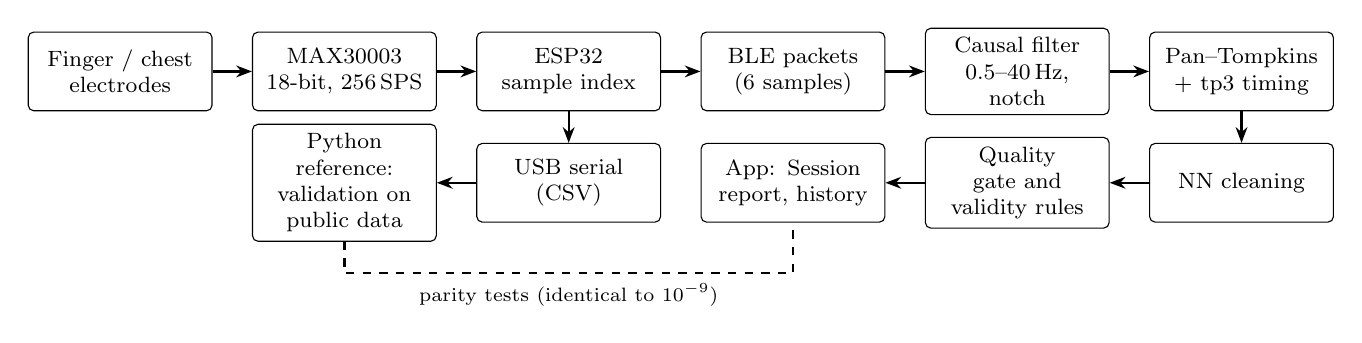
\begin{tikzpicture}[
  node distance=4mm and 5mm,
  blk/.style={draw,rounded corners=2pt,minimum height=10mm,text width=21mm,align=center,font=\footnotesize},
  arr/.style={-{Stealth[length=2mm]},thick}]
\node[blk] (el) {Finger / chest\\electrodes};
\node[blk,right=of el] (afe) {MAX30003\\18-bit, 256\,SPS};
\node[blk,right=of afe] (mcu) {ESP32\\sample index};
\node[blk,right=of mcu] (ble) {BLE packets\\(6 samples)};
\node[blk,right=of ble] (filt) {Causal filter\\0.5--40\,Hz, notch};
\node[blk,right=of filt] (det) {Pan--Tompkins\\+ tp3 timing};
\node[blk,below=of det] (nn) {NN cleaning};
\node[blk,left=of nn] (sqi) {Quality gate and validity rules};
\node[blk,left=of sqi] (out) {App: Session report, history};
\node[blk,below=of mcu] (usb) {USB serial\\(CSV)};
\node[blk,left=of usb] (py) {Python reference:\\validation on public data};
\draw[arr] (el)--(afe); \draw[arr] (afe)--(mcu); \draw[arr] (mcu)--(ble); \draw[arr] (ble)--(filt); \draw[arr] (filt)--(det); \draw[arr] (det)--(nn); \draw[arr] (nn)--(sqi); \draw[arr] (sqi)--(out);
\draw[arr] (mcu)--(usb); \draw[arr] (usb)--(py);
\draw[dashed,thick] (py.south) |- ++(0,-4mm) -| node[pos=0.25,below,font=\scriptsize]{parity tests (identical to $10^{-9}$)} (out.south);
\end{tikzpicture}
\caption{System architecture. The same filter, detector and analysis run live on the phone and offline in Python; parity tests force the two to agree.}
\label{fig:arch}
\end{figure*}

The system (Fig.~\ref{fig:arch}) has three parts: the hardware and firmware that acquire the ECG, the Android application that processes it in real time, and a Python toolchain that holds the reference implementation of every algorithm and validates it on public data.

\subsection{Reference Board}
The reference board is a custom PCB (Fig.~\ref{fig:schematic}) built around an ESP32-WROOM-32D module. Its MAX30003 ECG front end has a $\SI{49.9}{\kilo\ohm}$ series resistor and 10\,pF/1\,nF EMI filter on each input, and the common-mode output VCM is routed to the electrode connector as the body reference electrode. A SiT1533 32.768\,kHz oscillator clocks the MAX30003, so the sample rate is set by this crystal and not by the microcontroller. The board also carries a MAX30102 PPG sensor, a MAX30205 temperature sensor and an MPU6050 inertial sensor on a shared I$^2$C bus, and a galvanic skin response (GSR) front end built from LM324 op-amp stages feeding an ESP32 ADC input. Power comes from a DC input through AMS1117 3.3\,V and LD1117 1.8\,V regulators.

\begin{figure}[t]
\centering
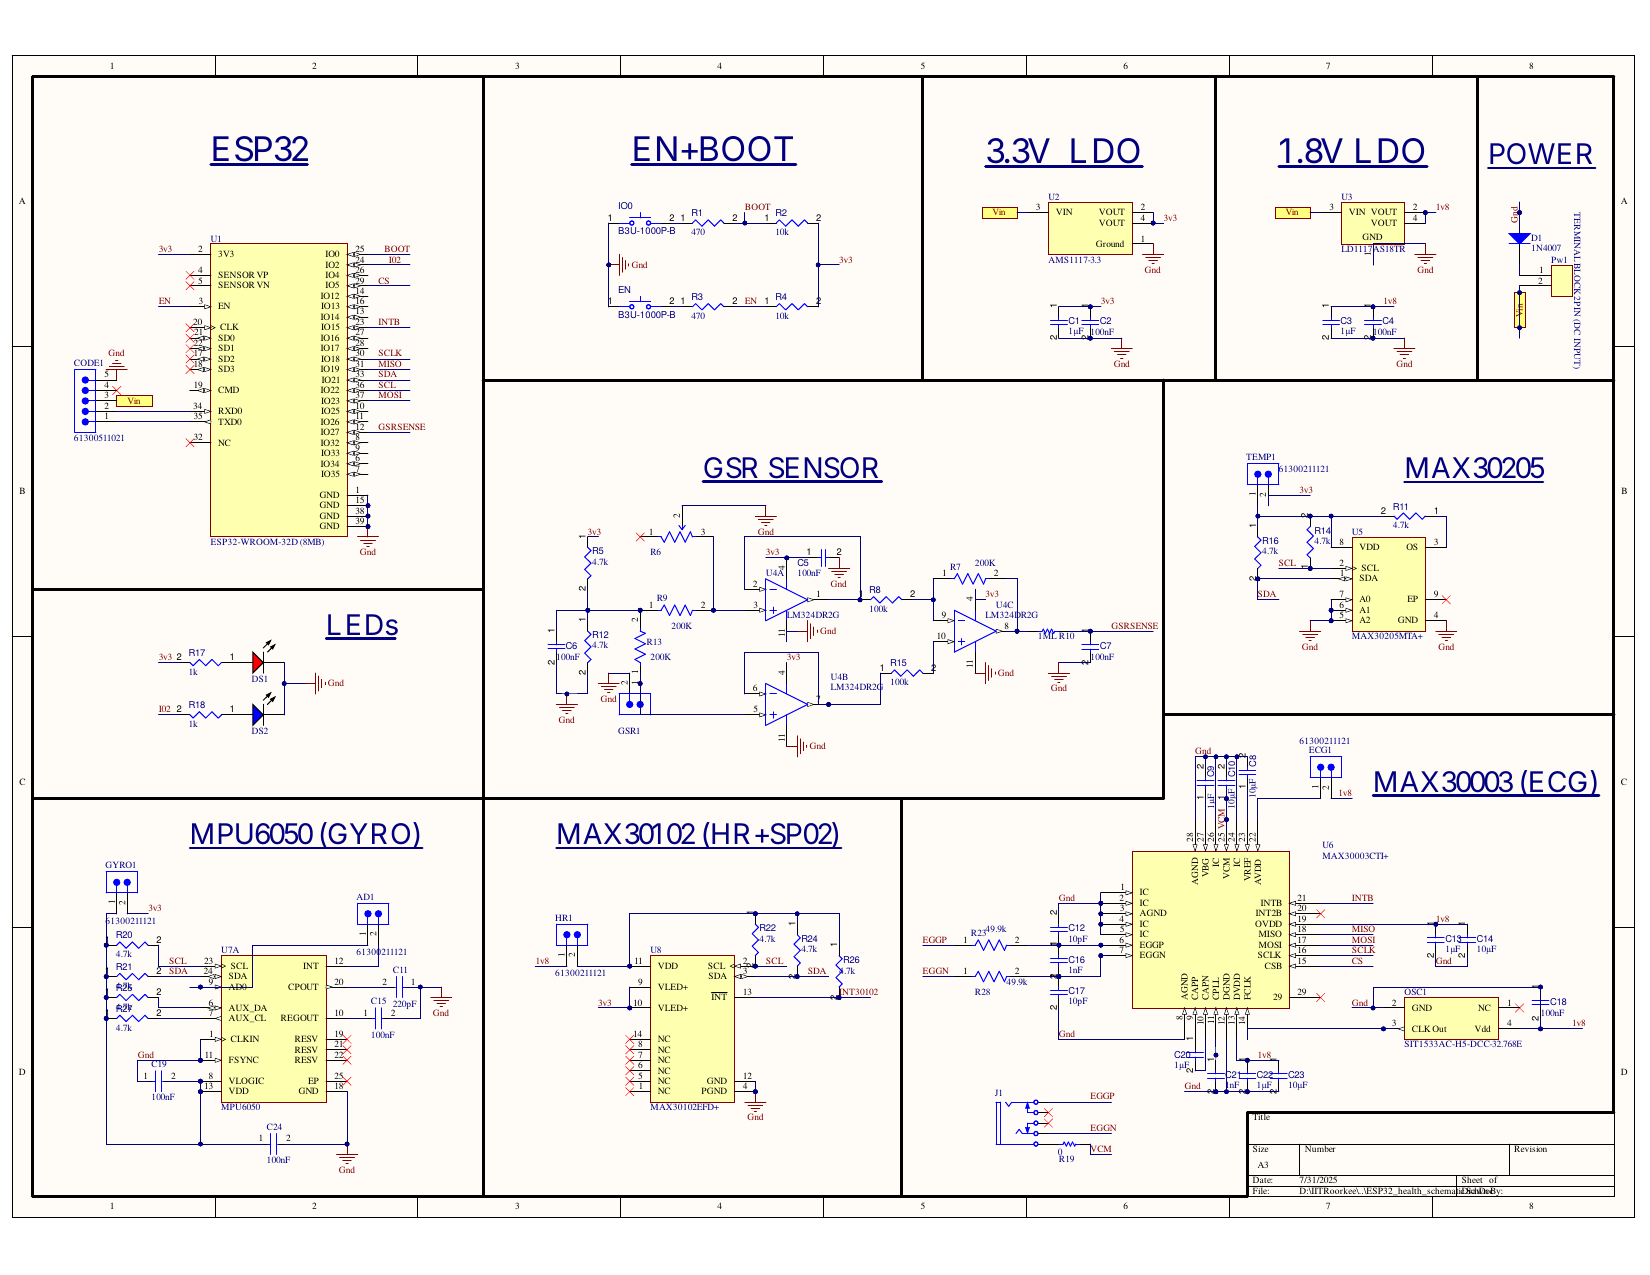
\includegraphics[width=\columnwidth]{figs/schematic-1.png}
\caption{Schematic of the reference board: ESP32-WROOM-32D, MAX30003 ECG front end, MAX30102 PPG, MAX30205 temperature, MPU6050 IMU, LM324 GSR front end and 3.3\,V/1.8\,V regulators.}
\label{fig:schematic}
\end{figure}

\subsection{Ring-Format Development Board}
The ring-format board pairs a MAX30003 with an ESP32-C3 SuperMini, which has native USB and BLE. It runs the same firmware as the reference board and sends data to the phone over BLE. \TODO{MAX30003 module/breakout used and electrode arrangement.} A further custom ESP32-C3 board with a U.FL antenna connector was used to test wireless stability.

\subsection{Flexible PCB for the Ring}
\TODO{Flex PCB: number of layers and stack-up; outline dimensions and ring size; component placement (MAX30003, ESP32-C3 or SoC, sensors, battery and charging); electrode design (inner ring electrode and outer touch electrode); antenna; design tool; fabrication house and date sent for fabrication.} The layout (Fig.~\ref{fig:flex}) has been sent for fabrication.

\begin{figure}[t]
\centering
\fbox{\parbox[c][35mm][c]{0.9\columnwidth}{\centering\TODO{Flex PCB layout image}}}
\caption{Flexible PCB layout of the ring. \TODO{caption details}}
\label{fig:flex}
\end{figure}

\subsection{Firmware}
The MAX30003 runs at 256 samples/s with a gain of 20\,V/V and raises an interrupt when four unread samples are in its FIFO. The ESP32 drains the FIFO, decodes each 24-bit word into an 18-bit signed sample and its ETAG status (valid, fast recovery, empty or overflow) \cite{max30003}, and assigns it a sample index. Sample $N$ was taken at $N/256$\,s on the front end's crystal; this index, rather than the host's clock, is used for all timing. Samples leave over USB as text lines and, on the ring-format board, over BLE in 20-byte notifications carrying a sequence number and six 3-byte samples (one packet every 23.4\,ms). The phone detects lost packets from the sequence number and tells the detector how many samples are missing, so that later beats keep their correct times. Both boards build from one source file, so decoding, register configuration, sample rate and timestamping are byte-identical and a finger-versus-chest difference can only come from the electrode site.

\subsection{Real-Time Signal Conditioning}
The phone filters each sample with a cascade of biquad sections: a fourth-order Butterworth high-pass at 0.5\,Hz, notches at 50 and 100\,Hz ($Q=30$) and a fourth-order Butterworth low-pass at 40\,Hz. The cascade is causal, with a measured delay of two samples (7.8\,ms); offline analyses use the same filter applied forwards and backwards (zero phase) as a best case.

\subsection{Beat Detection}
Beats are detected by a streaming Pan--Tompkins detector \cite{pantompkins}: a 5--15\,Hz band-pass, the five-point derivative $d[n]=\tfrac18(2x[n]+x[n-1]-x[n-3]-2x[n-4])$, squaring, 150\,ms moving-window integration and adaptive thresholds
\begin{equation}
\mathrm{THR}_1=\mathrm{NPK}+0.25(\mathrm{SPK}-\mathrm{NPK}),\qquad \mathrm{THR}_2=0.5\,\mathrm{THR}_1,
\end{equation}
with a 200\,ms refractory period, a T-wave check and search-back after $1.66\times$ the mean RR interval. Two additions were made: the signal level decays after 3\,s without a beat, so that an electrode transient cannot leave the threshold permanently too high, and search-back beats are located in the correct window. The detector is written sample by sample in Python and ported line for line to Kotlin.

\subsection{Beat Timing for HRV}
Detection only establishes that a beat occurred near a sample; HRV needs its time to a fraction of a sample. If each beat time carries an independent error of standard deviation $\sigma$, a successive RR difference carries $e_{i+2}-2e_{i+1}+e_i$, so
\begin{equation}
\mathrm{RMSSD}^2_{\text{meas}}\approx\mathrm{RMSSD}^2_{\text{true}}+6\sigma^2 .
\label{eq:jitter}
\end{equation}
Quantisation at 256\,Hz ($\sigma=3.9/\sqrt{12}=1.13$\,ms) adds only about 0.2\,ms to an RMSSD of 18\,ms. The conventional timing point, the maximum of the band-passed signal, behaves differently: under causal filtering it jumps between the two lobes of the QRS. The final timing point (tp3) instead aligns each beat with the median of the previous 16 beats. For lags $\ell$ within $\pm10$ samples it computes the correlation $r(\ell)$ between the detrended beat window and the template, takes the best lag $\ell^\ast$ with parabolic sub-sample refinement, and accepts the beat only if $r(\ell^\ast)\ge0.8$ and $\ell^\ast$ is inside the range. All beats are thereby timed at the same point of the waveform, with no decision about polarity.

\subsection{HRV, Breathing and Rhythm Analysis}
RR intervals are cleaned to normal-to-normal (NN) intervals: an interval differing by more than 20\% from the previous accepted one is dropped, and no difference is taken across a dropped interval or a data gap. Each measure is reported only when its minimum amount of valid data is present (Table~\ref{tab:minwin}); otherwise the app states the reason. LF and HF power are integrated from the Lomb--Scargle periodogram of the NN series and are withheld below 95\% beat coverage: in simulation HF read $+15.9\%$ and $+30.3\%$ high at about 90\% coverage, hence the 95\% rule.

\begin{table}[t]
\centering
\caption{Minimum valid NN time before a measure is reported}
\label{tab:minwin}
\footnotesize\setlength{\tabcolsep}{4pt}
\begin{tabular}{@{}ll@{}}
\toprule
Measure & Minimum \\
\midrule
RMSSD, pNN50, SD1 & 60\,s and 30 intervals \\
HF & 60\,s at $\geq$95\% coverage \\
SDNN, SD2 & 120\,s \\
LF, LF/HF & 120\,s at $\geq$95\% coverage \\
DFA $\alpha_1$ (boxes of 4--16 beats \cite{peng1995}) & 120\,s and 200 intervals \\
Sample entropy ($m=2$, $r=0.2\,\mathrm{SD}$) & 180\,s and 200 templates \\
\bottomrule
\end{tabular}
\end{table}

Breathing rate is estimated in 32\,s windows from two modulations of the ECG, respiratory sinus arrhythmia in the NN series and the R-wave amplitude, as the dominant Lomb--Scargle peak between 4 and 40 breaths/min; a fused rate is reported when the two estimates agree within 3 breaths/min, or from the R-wave amplitude alone when its peak holds at least 40\% of the band's power, and never from respiratory sinus arrhythmia alone. Ventricular ectopic beats are labelled from two features: the correlation of each beat with a template of recent normal beats, and its prematurity relative to recent normal intervals. The AF screen computes eleven RR-irregularity features over 30\,s, including normalised RMSSD, the Poincar\'e ratio SD1/SD2, the turning-point ratio and the coefficient of sample entropy \cite{lake2011}, and classifies them with 100 gradient-boosted trees of depth~3; the choice of model was fixed before evaluation.

\subsection{Signal Quality}
Every 5\,s the app grades the signal from the kurtosis of the displayed signal (kSQI) and the share of its energy in the 5--15\,Hz QRS band (pSQI) \cite{li2008}: GOOD when kSQI\,$\geq5$ and pSQI\,$\geq0.10$, FAIR when kSQI\,$\geq3.5$ and pSQI\,$\geq0.05$. Because kurtosis rewards any spike, an artifact check marks the signal POOR for 10\,s when a 1\,s block swings more than four times the median of the last 30 blocks. Heart rate is displayed only on GOOD.

\subsection{Android Application}
The application (Fig.~\ref{fig:app}) is written in Kotlin with Jetpack Compose. A ViewModel owns the BLE client and the processing pipeline, so both survive screen rotation, and reconnects after a dropped link. The live monitor draws the ECG on paper ruled in true millimetres (25\,mm/s) computed from the screen's physical density, with the live heart rate taken from located beats in the last 10\,s. A three-minute Session (five minutes in an extended mode that adds DFA $\alpha_1$ and sample entropy) produces a report of heart rate, breathing rate and HRV, each with its coverage, stored in an on-device database with a personal baseline after three sessions. A guided-breathing screen paces breathing at six breaths per minute with live HRV. A replay mode feeds saved recordings through the same packet path.

\begin{figure}[t]
\centering
\begin{subfigure}{0.24\columnwidth}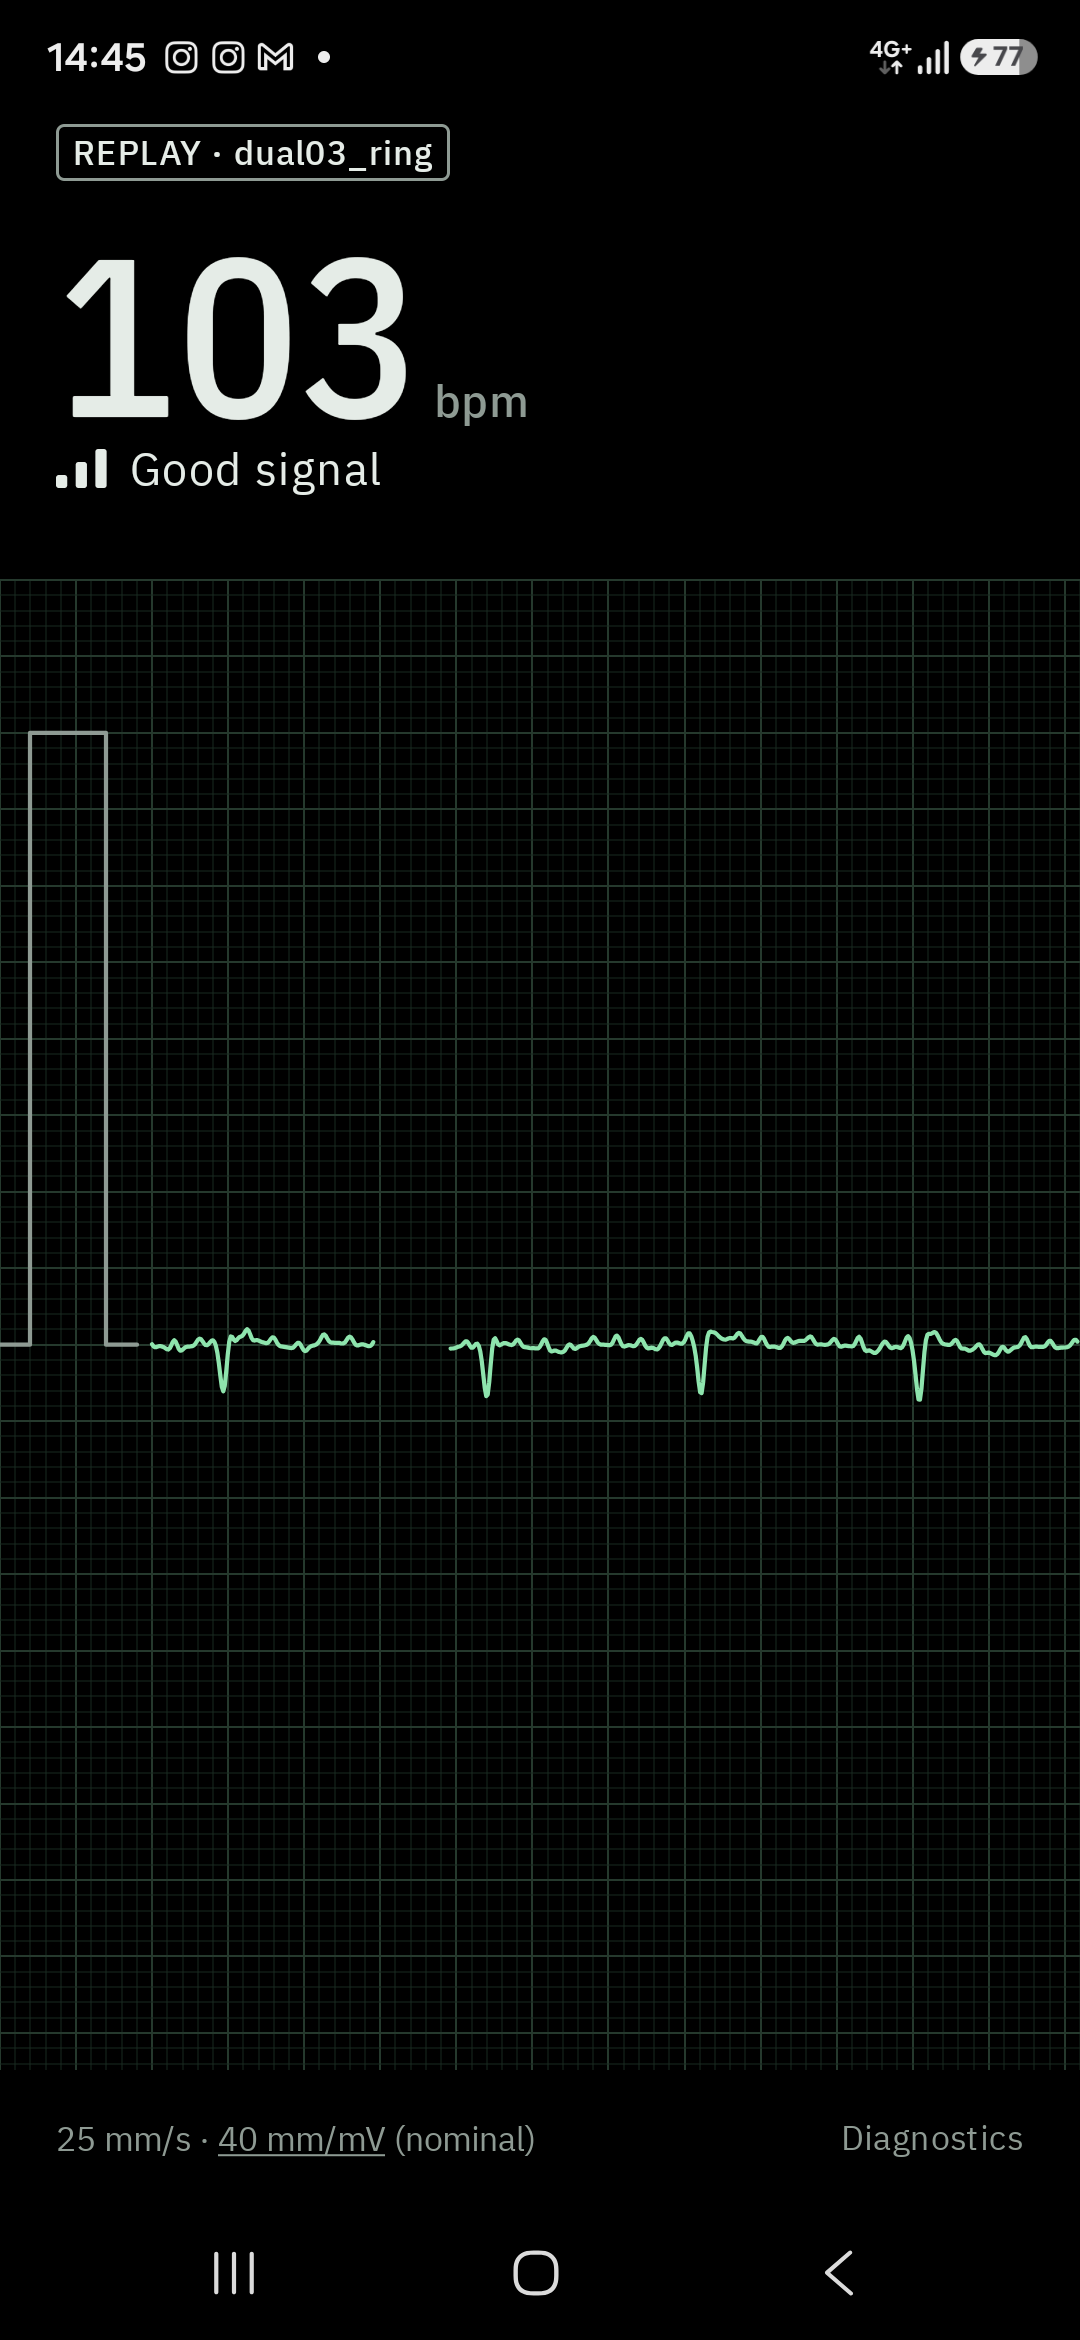
\includegraphics[width=\linewidth]{figs/app_monitor.png}\caption{}\end{subfigure}\hfill
\begin{subfigure}{0.24\columnwidth}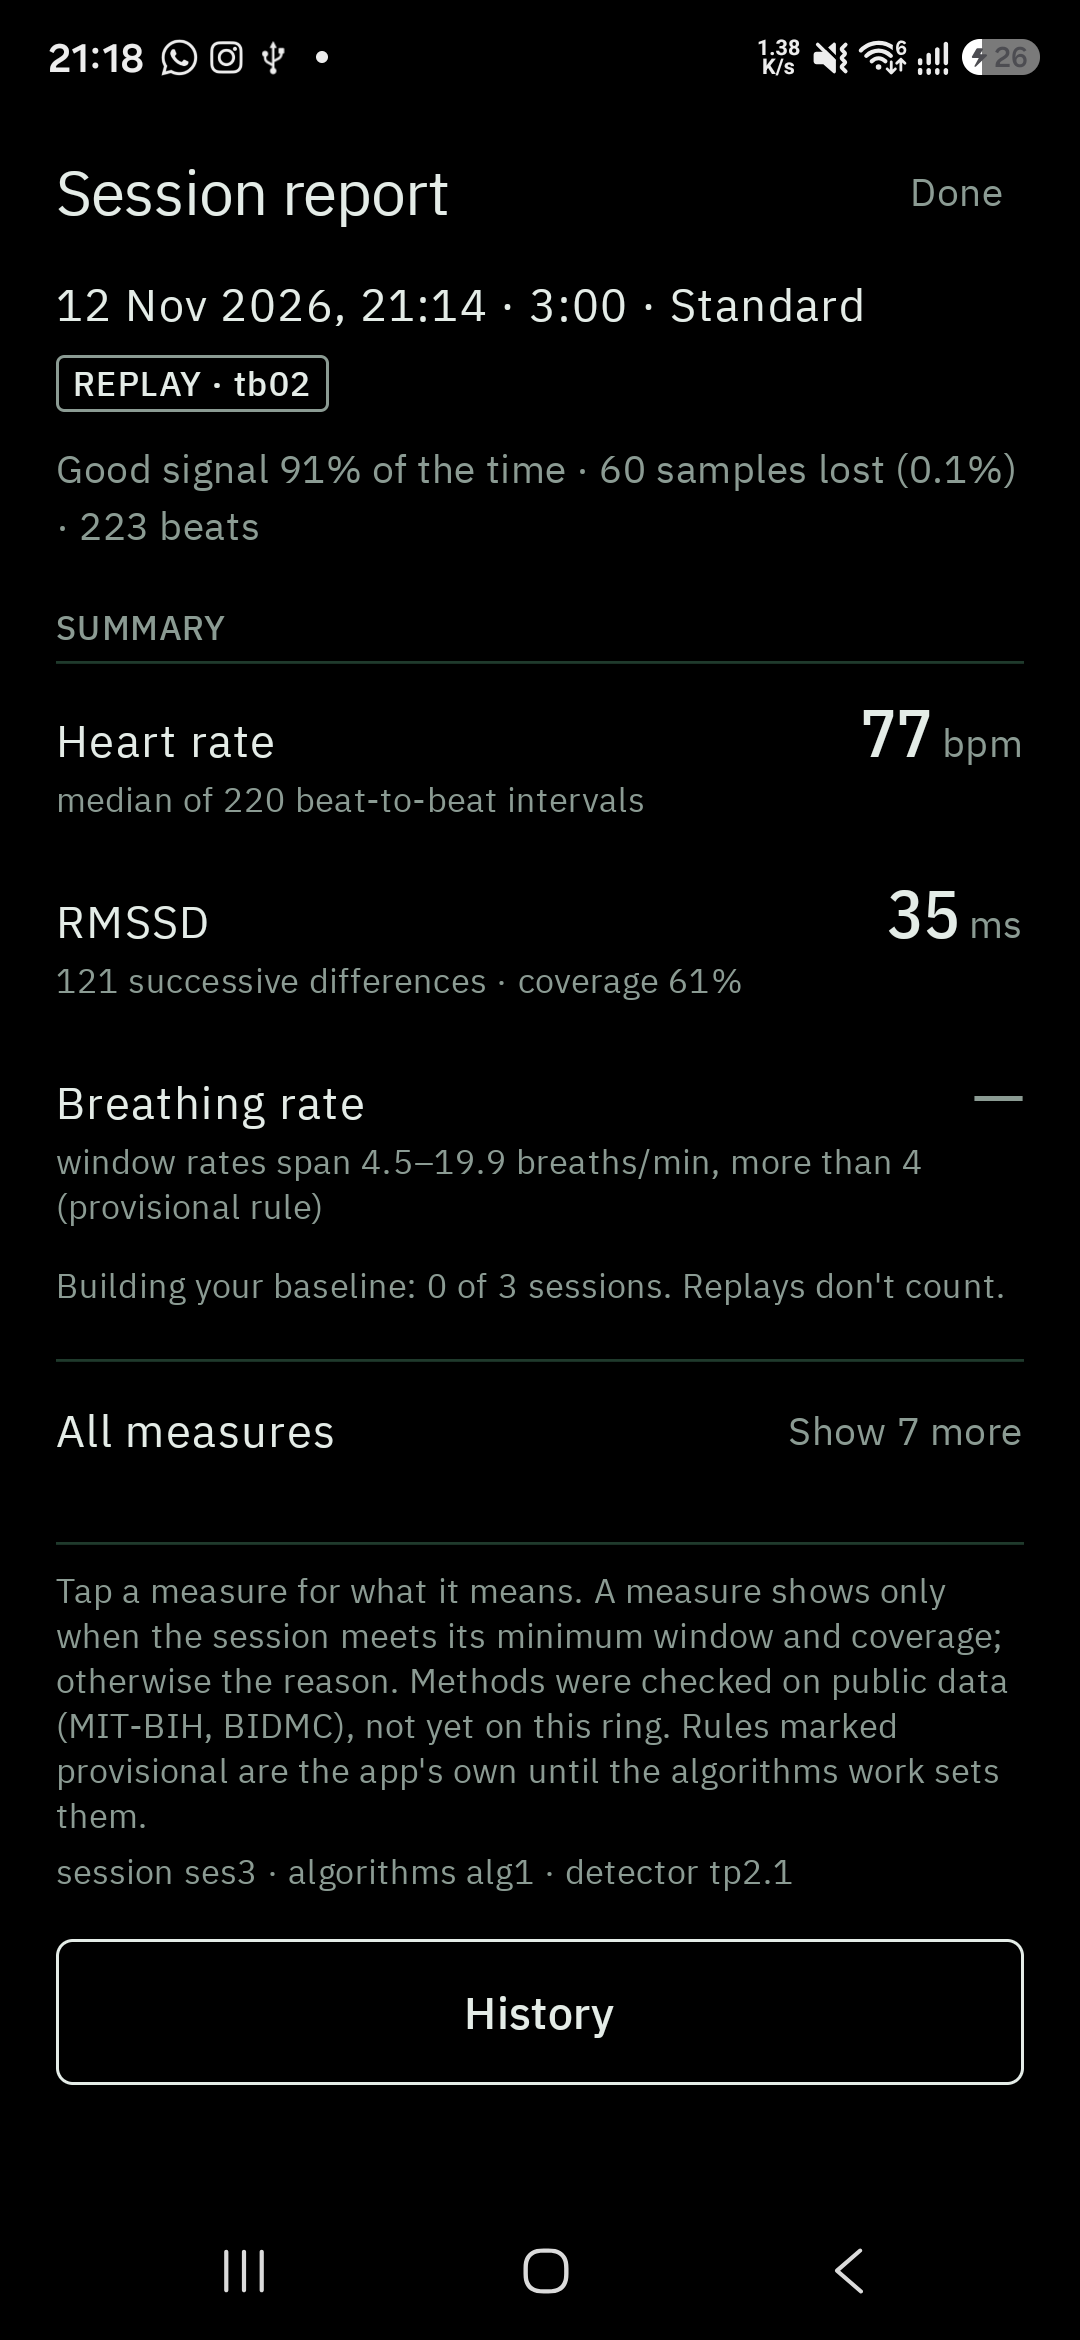
\includegraphics[width=\linewidth]{figs/app_report.png}\caption{}\end{subfigure}\hfill
\begin{subfigure}{0.24\columnwidth}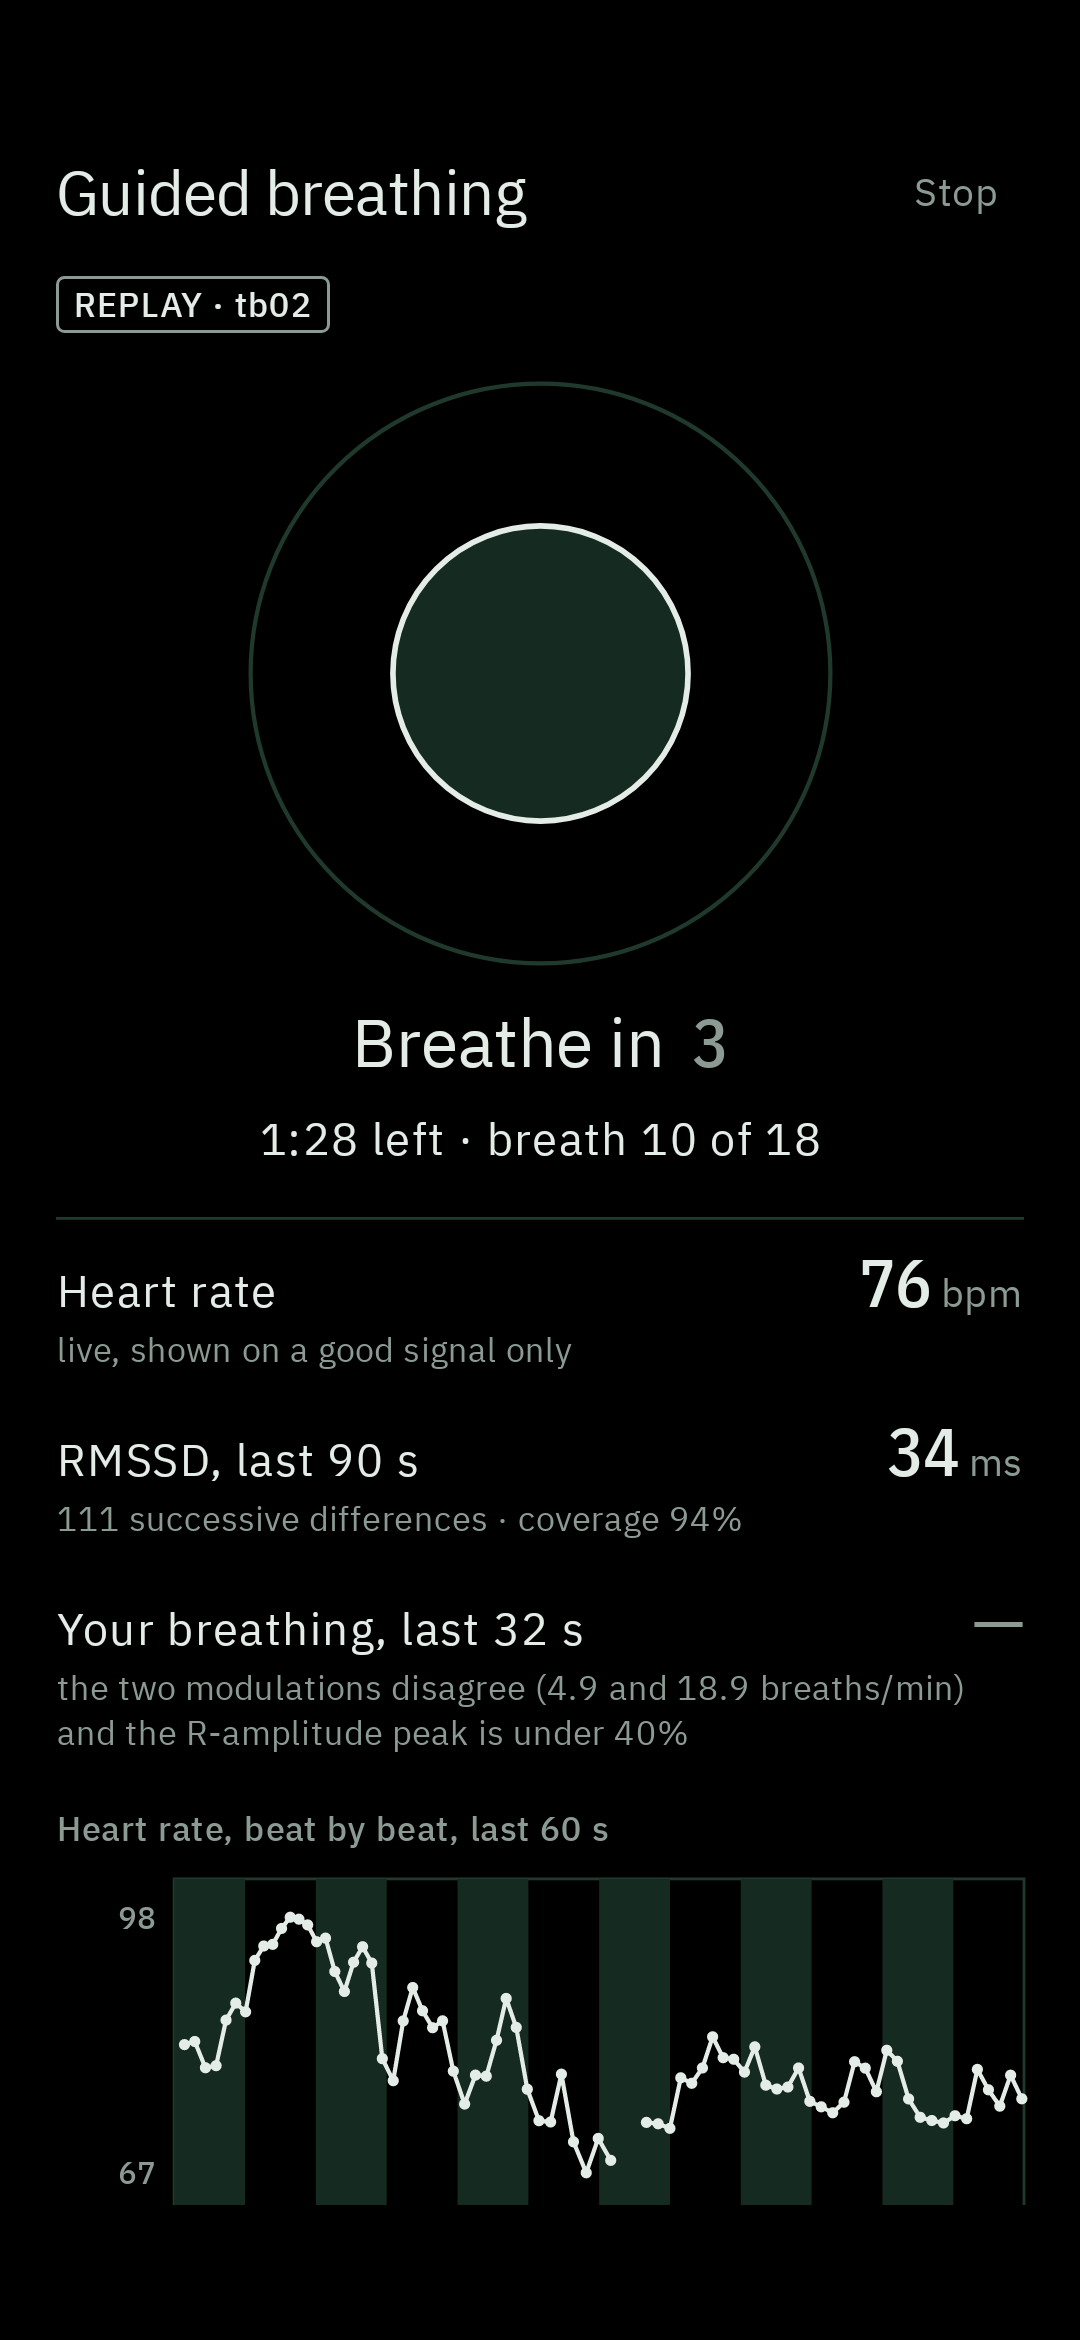
\includegraphics[width=\linewidth]{figs/app_breathing.png}\caption{}\end{subfigure}\hfill
\begin{subfigure}{0.24\columnwidth}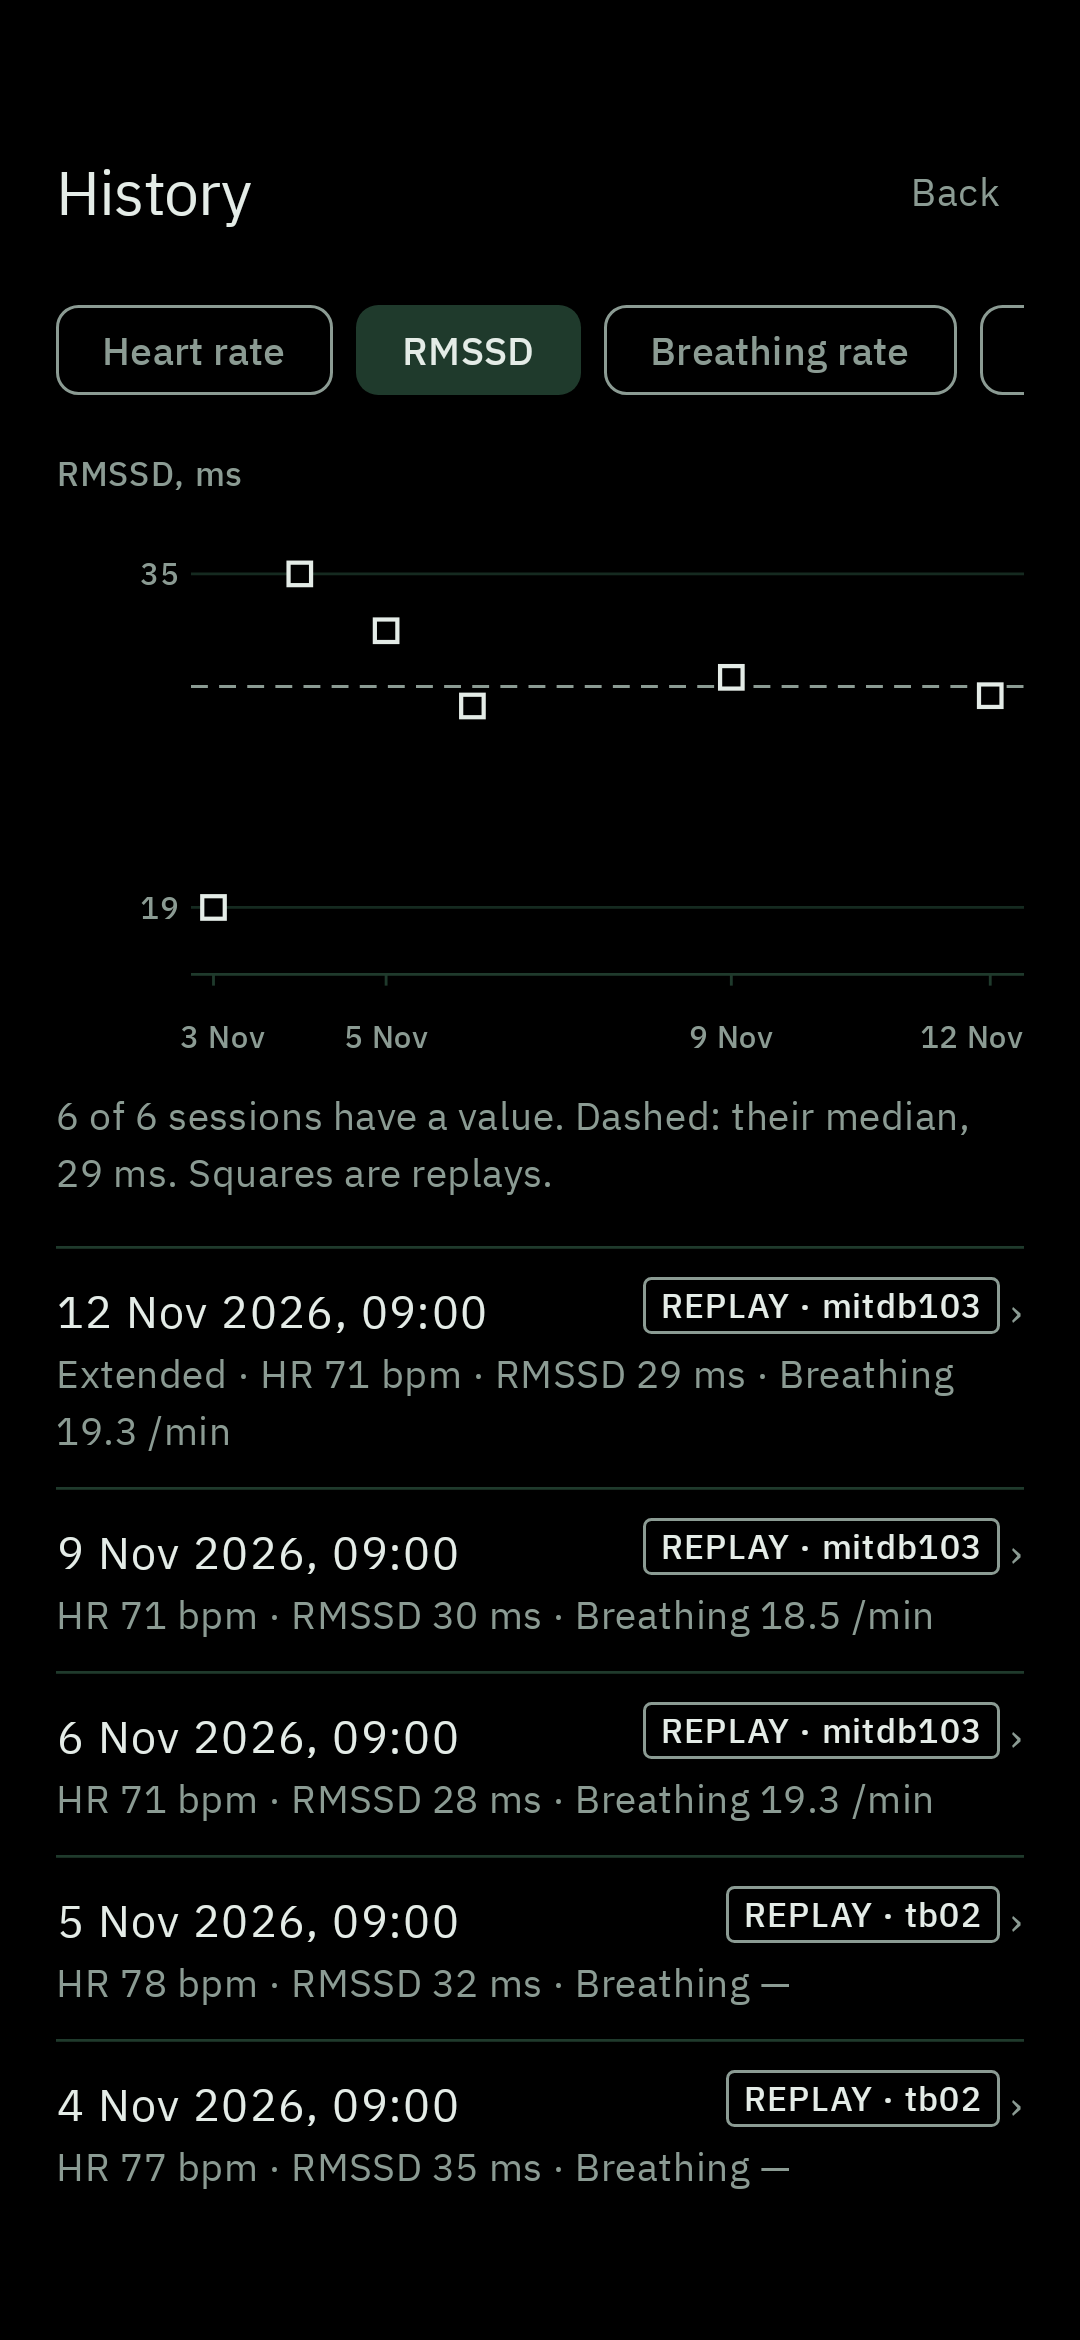
\includegraphics[width=\linewidth]{figs/app_history.png}\caption{}\end{subfigure}
\caption{Android application: (a) live monitor on millimetre ECG paper, (b) Session report, (c) guided breathing at six breaths/min, (d) history with personal baseline.}
\label{fig:app}
\end{figure}

\subsection{Verification and Validation Method}
Python is the reference implementation. Every algorithm on the phone is tested against it on real recordings and must agree to $10^{-9}$; the Android test suite (156 tests) also checks that every constant matches the frozen configuration, that the app's packet path gives the same beats as the detector alone, and that the live heart rate agrees with R peaks found independently by NeuroKit2 \cite{neurokit2}. For each algorithm, parameters were tuned on development data, frozen in a version-controlled commit, and then run once on held-out data: 36 MIT-BIH records \cite{mitbih}, the INCART database \cite{physionet}, held-out BIDMC subjects \cite{pimentel2017}, the MIT-BIH AF Database \cite{moody1983} and leave-one-subject-out testing on WESAD \cite{schmidt2018}. The ectopic-beat rule was tested on the de~Chazal DS2 set \cite{dechazal2004}, a separate set of patients; the detector underneath was developed on all of MIT-BIH. Every number reported below is generated by a script and saved with its settings; the results quoted are listed with their source files at repository tag \texttt{phase1-report-v2}.

% -------------------------------------------------------------
\section{Work Completed and Results}

\subsection{Acquisition Integrity}
A three-minute simultaneous capture from both boards, checked on the host for index continuity and duplicates, contained 44,548 samples from the ring-format board and 44,545 from the reference board, with 0 missing, 0 gaps and 0 duplicates. With no electrodes connected, the measured noise of the ring-format board was 1.42 codes rms, against 1.39 codes for the typical noise in the MAX30003 datasheet \cite{max30003}, converted on the nominal scale, which is not yet verified.

\subsection{Beat Detection}
Table~\ref{tab:ec57} gives EC57 results at 256\,Hz. On the 32 non-paced MIT-BIH records held out from development, with parameters frozen beforehand and the timing point then in use (tp2.1), the detector reached Se 99.78\% and P+ 99.32\%. With a two-detector agreement gate (bSQI\,$\geq0.9$), Se rose to 99.82\% and P+ to 99.89\% with 2.4\% of the data rejected. Correcting the search-back localisation raised the development figures from 98.50/97.31\% to 99.52/98.32\%. The beat-timing change (tp3) does not alter detection.

\begin{table}[t]
\centering
\caption{QRS Detection, ANSI/AAMI EC57, 150\,ms Tolerance, 256\,Hz}
\label{tab:ec57}
\footnotesize\setlength{\tabcolsep}{4pt}
\begin{tabular}{@{}llrr@{}}
\toprule
Detector & Records & Se (\%) & P+ (\%) \\
\midrule
Initial version & 12 development & 98.50 & 97.31 \\
NeuroKit2 \cite{neurokit2} (360\,Hz) & 12 development & 98.90 & 99.25 \\
Final (tp3) & 12 development & 99.49 & 98.29 \\
Final (tp2.1) & \textbf{32 held-out} & \textbf{99.78} & \textbf{99.32} \\
\quad with bSQI gate (2.4\% rej.) & 32 held-out & 99.82 & 99.89 \\
Final (tp2.1) & 4 held-out, paced & 99.55 & 99.24 \\
\bottomrule
\end{tabular}
\end{table}

\subsection{Finger Versus Chest on Identical Hardware}
Finger and chest ECG were recorded simultaneously at rest for 105\,s, the finger channel with one electrode on each hand and a reference electrode, the chest channel on the other board. The two recordings, which share no clock, were aligned by cross-correlating their beat trains. Treating the chest as reference, 178 of 179 beats were matched (Se\,=\,P+\,=\,99.44\%). Table~\ref{tab:agree} and Fig.~\ref{fig:agree} give the agreement, computed with the earlier timing point tp2; Section~\ref{sec:timing} gives the RR and RMSSD agreement with tp3. In bench tests, mains interference dominated the finger channel without the reference electrode, so the reference electrode is required.

\begin{table}[t]
\centering
\caption{Finger Versus Chest Agreement (Rest, 105\,s, Timing Point tp2)}
\label{tab:agree}
\footnotesize\setlength{\tabcolsep}{4pt}
\begin{tabular}{@{}ll@{}}
\toprule
Measure & Result \\
\midrule
Heart-rate bias & $+0.03$\,bpm \\
Heart-rate limits of agreement \cite{blandaltman} & $-0.10$ to $+0.15$\,bpm \\
ICC(2,1) / CCC \cite{lin1989} & 0.9998 / 0.9997 \\
RR intervals (169) & bias 0.00\,ms, LoA $\pm1.6$\,ms \\
RMSSD, cleaned NN & chest 18.1\,ms, finger 18.0\,ms \\
\bottomrule
\end{tabular}
\end{table}

\begin{figure}[t]
\centering
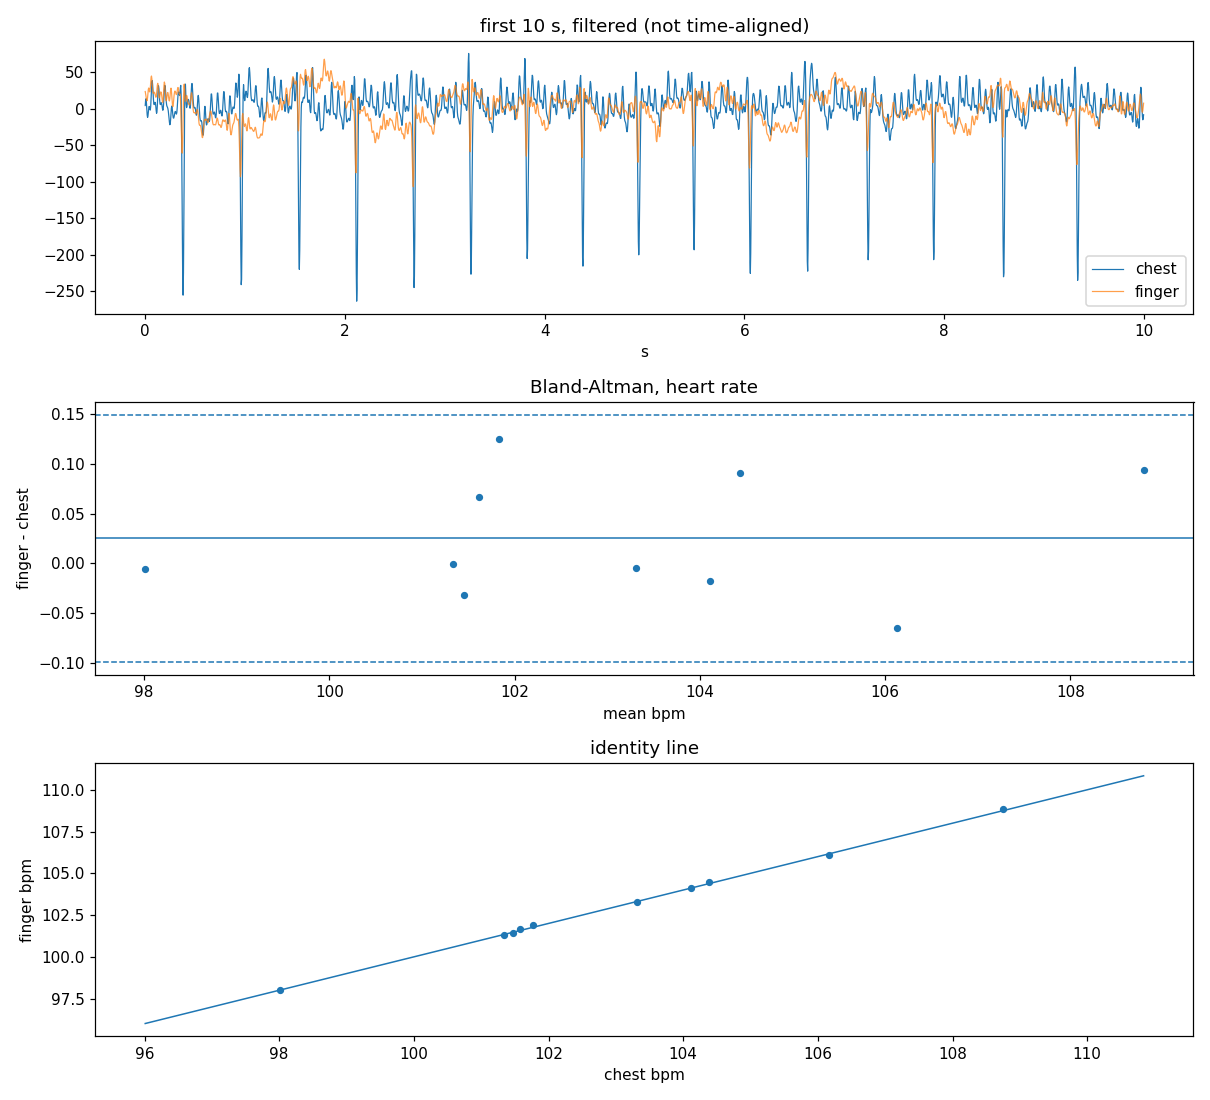
\includegraphics[width=\columnwidth]{figs/agreement_dual03.png}
\caption{Simultaneous finger and chest recording: filtered signals (top), Bland--Altman plot of heart rate (middle) and identity plot (bottom). Beats timed with tp2.}
\label{fig:agree}
\end{figure}

\subsection{Beat Timing Under Real-Time Filtering}
\label{sec:timing}
With the conventional timing point and the phone's causal filter, the beat time jumped between QRS lobes: on 48 of 179 matched beats the finger-minus-chest beat time was more than 20\,ms off, from $-39$ to $+35$\,ms (Fig.~\ref{fig:fiducial}). The finger RMSSD read 36.7\,ms while the chest, timed with tp3, read 18.3\,ms (coverage 92\%); by \eqref{eq:jitter} this corresponds to an effective timing error of about 13\,ms. With template-alignment timing (tp3) the finger RMSSD was 17.9\,ms (coverage 94\%, Fig.~\ref{fig:rmssd}) and the finger-versus-chest RR limits of agreement narrowed from $-37.6$\ldots$+37.5$\,ms to $\pm1.8$\,ms. On the INCART database, never used in development, the number of patients with less than 50\% usable intervals fell from 11 to 2 of 32, and the range of per-patient RMSSD errors narrowed from $-32.9$\ldots$+8.8$\,ms to $-6.5$\ldots$0.0$\,ms. Against MIT-BIH annotations (44 non-paced records, development data) the median RMSSD error of tp3 on the phone's filter was $-0.15$\,ms (range $-2.27$ to $+3.45$\,ms).

\begin{figure}[t]
\centering
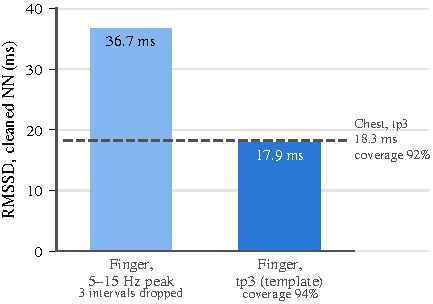
\includegraphics[width=0.9\columnwidth]{figs/rmssd_timing_fix.pdf}
\caption{Finger RMSSD on the simultaneous recording under the phone's causal filter, with beats timed at the 5--15\,Hz peak and with tp3; the dashed line is the chest RMSSD with tp3. Cleaned NN series, coverage below each bar.}
\label{fig:rmssd}
\end{figure}

\begin{figure*}[t]
\centering
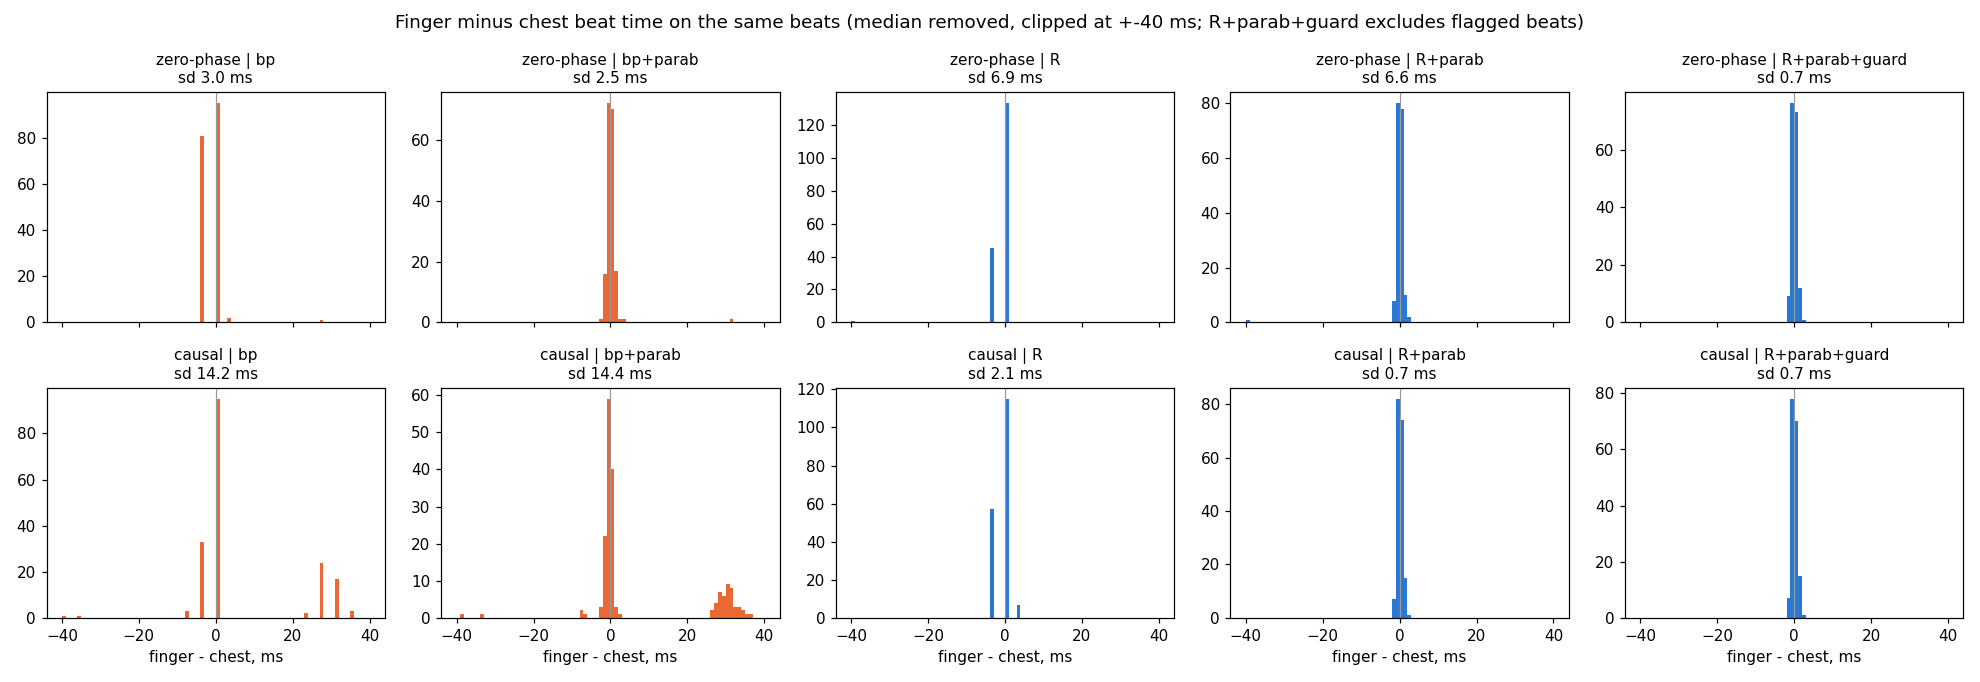
\includegraphics[width=\textwidth]{figs/fiducial_v2.png}
\caption{Finger minus chest beat time on the same beats for five timing points, zero-phase (top) and causal (bottom) filtering. The band-passed peak (left two columns) splits into two clusters under causal filtering (lobe-jumping); timing on the R peak with parabolic interpolation (right) keeps the spread below 1\,ms.}
\label{fig:fiducial}
\end{figure*}

\subsection{HRV Implementation}
Given identical NN series (beats timed with tp2.1), the HRV functions matched NeuroKit2 \cite{neurokit2} on the 192 held-out five-minute MIT-BIH windows: RMSSD and SD1 identically in the 182 windows where they were reported, SDNN and SD2 in 178; DFA $\alpha_1$ and sample entropy identical (to $10^{-14}$) on the 15 windows without holes; and LF/HF within 3.2\% on windows without holes and 4.7\% on windows with holes (0.03\% and 0.15\% on NeuroKit2's frequency grid).

\subsection{Breathing Rate, Ectopic Beats and AF}
Table~\ref{tab:analytics} summarises the analyses tested on data not used to tune them. Breathing rate was tuned on half of the BIDMC subjects and tested once on the other half. Ventricular ectopic beats were tuned on the de~Chazal DS1 records and tested on DS2, a separate set of patients; the detector underneath was developed on all of MIT-BIH. The AF screen was developed on CinC 2017 \cite{clifford2017} by cross-validation (5 folds $\times$ 3 repeats; F1 0.871 normal, 0.735 AF, 0.644 other rhythm) and tested once on 23 patients of the MIT-BIH AF Database, where 97.2\% of 30\,s windows were judged and the per-patient median sensitivity was 98.1\%.

\begin{table}[t]
\centering
\caption{Analytics Tested on Data Not Used to Tune Them}
\label{tab:analytics}
\footnotesize\setlength{\tabcolsep}{4pt}
\begin{tabular}{@{}lll@{}}
\toprule
Analysis & Test data & Result \\
\midrule
Breathing rate & BIDMC, 23 held-out & MAE 0.50\,br/min \\
 & subjects & LoA $-2.9$ to $+3.3$ \\
 & & 41\% of windows \\
\addlinespace
Ventricular & MIT-BIH DS2 & Se 88.4\%, P+ 82.7\% \\
ectopic beats & (separate patients) & F1 85.4, cov. 98.6\% \\
\addlinespace
AF screen & MIT-BIH AF Database & Se 92.2\%, Sp 96.8\% \\
 & (external, 23 patients) & cov. 97.2\% \\
\bottomrule
\end{tabular}
\end{table}

\subsection{Multi-Sensor Arousal}
A multi-sensor arousal model was specified in advance, with two amendments approved before any classification metric was computed, and evaluated once with leave-one-subject-out testing on WESAD \cite{schmidt2018} (15 subjects). Windows of 180\,s were described by ECG time-domain HRV, wrist pulse rate and amplitude, EDA tonic level and skin-conductance responses (cvxEDA \cite{greco2016}) and skin-temperature slope, each z-scored against the subject's own baseline, and classified by logistic regression. Table~\ref{tab:wesad} and Fig.~\ref{fig:wesad} give stress-versus-rest results. EDA carries most of the information; skin temperature alone is weak. On the binary task of the original study (stress versus baseline plus amusement), the wrist-only model reached 90.4\% accuracy on the windows it classified, with 13.1\% of stress and 10.5\% of non-stress windows rejected, against 88.33\% reported for wrist signals and 93.12\% for chest signals in \cite{schmidt2018}, with different windows and classifiers.

\begin{table}[t]
\centering
\caption{Stress Versus Rest on WESAD, Leave-One-Subject-Out}
\label{tab:wesad}
\footnotesize\setlength{\tabcolsep}{4pt}
\begin{tabular}{@{}lccc@{}}
\toprule
Model & Bal. acc. (\%) & Se / Sp (\%) & Rejected \\
\midrule
All four signals & 96.1 & 92.2 / 100.0 & 13.1\% \\
Wrist only & 93.3 & 88.5 / 98.0 & 13.1\% \\
EDA alone & 87.2 & 80.1 / 94.3 & 0\% \\
Temperature alone & 64.9 & 54.2 / 75.7 & 0\% \\
\bottomrule
\end{tabular}
\\[2pt]{\footnotesize Rejected: share of stress windows lacking a required feature; the same models also rejected 5.2\% of baseline windows. 95\% intervals over subjects: 91.8--100 (all four), 84.2--99.3 (wrist).}
\end{table}

\begin{figure}[t]
\centering
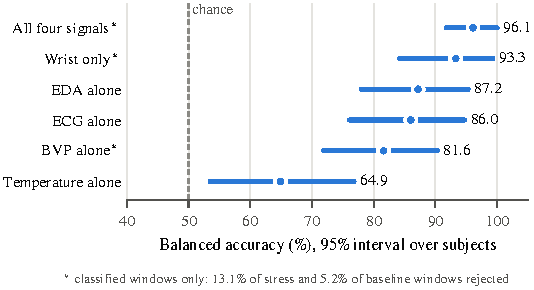
\includegraphics[width=\columnwidth]{figs/wesad_balacc.pdf}
\caption{Stress versus rest on WESAD, leave-one-subject-out: balanced accuracy with 95\% intervals from a bootstrap over the 15 subjects. Starred models are scored on classified windows only.}
\label{fig:wesad}
\end{figure}

\subsection{Application}
All 156 Android tests pass at the reported version, with the phone's HRV, breathing, detector and quality-gate outputs identical to the Python reference to $10^{-9}$. The live heart-rate display, compared with R peaks found independently on two recordings, was never more than 5\,bpm off at any of 1,359 displayed moments. The artifact check reduced the share of GOOD verdicts during an electrode-settling transient from 47.8\% to 2.5\% without rejecting any window of the 48 MIT-BIH records previously graded GOOD. The ECG grid drawn on a Samsung Galaxy A56 matched 5\,mm to within one pixel in both orientations.

% -------------------------------------------------------------
\section{Discussion and Current Limitations}

\subsection{Discussion of Results}
The detector performs at the level expected of a classical Pan--Tompkins design while running at the device's 256\,Hz and remaining identical between Python and the phone. The finger-versus-chest comparison shows that, on identical hardware, the finger site reproduces chest heart rate and RR intervals within a few milliseconds. The main technical finding concerns beat timing: under the causal filtering a phone must use, the conventional timing point is not merely noisy but two-valued, and \eqref{eq:jitter} explains why this doubled RMSSD while leaving heart rate unaffected. Timing each beat by its alignment with a running template removes the effect without a polarity decision and holds on a database not used in development. The validity windows and quality gate let the application withhold, rather than estimate, any value its data cannot support.

\subsection{Current Limitations and Planned Fixes}
Table~\ref{tab:limits} lists the main limitations, each with the step that will address it.

\begin{table}[t]
\centering
\caption{Current Limitations and Planned Fixes}
\label{tab:limits}
\begin{tabular}{@{}p{0.47\columnwidth}p{0.45\columnwidth}@{}}
\toprule
Limitation & Planned fix \\
\midrule
Finger--chest agreement from one subject at rest. & Multi-subject study at rest and in light motion. \\
\addlinespace
Ring not yet assembled. & Bring-up of the fabricated flex PCB. \\
\addlinespace
Arousal, AF and ectopic analyses validated on public data. & Evaluation on recordings from the ring and reference board. \\
\addlinespace
Signal amplitude lower than expected; input configuration under test. & Front-end configuration test; quote amplitudes in mV once calibrated. \\
\bottomrule
\end{tabular}
\end{table}

% -------------------------------------------------------------
\section{Conclusion and Proposed Work for Phase II}
An ECG acquisition platform for a finger-electrode ring, with identical firmware on a ring-format and a reference board, a real-time Android application and a Python reference, was built and validated link by link. The detector reached 99.78\% sensitivity and 99.32\% positive predictivity on held-out MIT-BIH records, and finger and chest heart rate agreed within $-0.10$ to $+0.15$\,bpm. Real-time filtering was shown to make the conventional beat-timing point jump between QRS lobes, doubling RMSSD; a template-alignment timing point corrects this and generalises to unseen data. On this foundation the system reports HRV, breathing rate, ectopic beats and an AF screen, each tested on data not used to tune it, and a pre-specified multi-sensor arousal model reaches 93.3\% balanced accuracy from wrist-type signals.

Phase~II will assemble and bring up the flexible-PCB ring; integrate the PPG, skin-conductance, temperature and motion sensors into the data stream, including pulse arrival time from the shared clock; move the AF screen and ectopic-beat count into the application; and carry out a multi-subject validation study of the ring against chest ECG. \TODO{Phase~II SoC test work, if part of the project.}

% -------------------------------------------------------------
\begin{thebibliography}{99}\small
\bibitem{briosa2025} A. Briosa e Gala \textit{et al.}, ``Diagnostic performance of single-lead electrocardiograms from the Apple Watch and CART Ring for cardiac arrhythmias,'' \textit{Heart Rhythm O2}, 2025, doi: 10.1016/j.hroo.2025.03.019.
\bibitem{mahajan2025} S. Mahajan \textit{et al.}, ``Evaluation of Spandan smartphone-based electrocardiogram for arrhythmia detection: A cross-sectional study in a large patient cohort,'' \textit{Anatol. J. Cardiol.}, vol. 29, no. 5, pp. 228--241, 2025.
\bibitem{pantompkins} J. Pan and W. J. Tompkins, ``A real-time QRS detection algorithm,'' \textit{IEEE Trans. Biomed. Eng.}, vol. BME-32, no. 3, pp. 230--236, Mar. 1985.
\bibitem{ec57} ANSI/AAMI EC57:2012, \textit{Testing and Reporting Performance Results of Cardiac Rhythm and ST Segment Measurement Algorithms}. Arlington, VA, USA: AAMI, 2012.
\bibitem{mitbih} G. B. Moody and R. G. Mark, ``The impact of the MIT-BIH Arrhythmia Database,'' \textit{IEEE Eng. Med. Biol. Mag.}, vol. 20, no. 3, pp. 45--50, 2001.
\bibitem{physionet} A. L. Goldberger \textit{et al.}, ``PhysioBank, PhysioToolkit, and PhysioNet,'' \textit{Circulation}, vol. 101, no. 23, pp. e215--e220, 2000.
\bibitem{taskforce} Task Force of the ESC and NASPE, ``Heart rate variability: Standards of measurement, physiological interpretation and clinical use,'' \textit{Circulation}, vol. 93, no. 5, pp. 1043--1065, 1996.
\bibitem{peng1995} C.-K. Peng, S. Havlin, H. E. Stanley, and A. L. Goldberger, ``Quantification of scaling exponents and crossover phenomena in nonstationary heartbeat time series,'' \textit{Chaos}, vol. 5, no. 1, pp. 82--87, 1995.
\bibitem{richman2000} J. S. Richman and J. R. Moorman, ``Physiological time-series analysis using approximate entropy and sample entropy,'' \textit{Am. J. Physiol. Heart Circ. Physiol.}, vol. 278, no. 6, pp. H2039--H2049, 2000.
\bibitem{lomb} N. R. Lomb, ``Least-squares frequency analysis of unequally spaced data,'' \textit{Astrophys. Space Sci.}, vol. 39, pp. 447--462, 1976.
\bibitem{scargle} J. D. Scargle, ``Studies in astronomical time series analysis. II,'' \textit{Astrophys. J.}, vol. 263, pp. 835--853, 1982.
\bibitem{munoz2015} M. L. Munoz \textit{et al.}, ``Validity of (ultra-)short recordings for heart rate variability measurements,'' \textit{PLoS ONE}, vol. 10, no. 9, e0138921, 2015.
\bibitem{shaffer2017} F. Shaffer and J. P. Ginsberg, ``An overview of heart rate variability metrics and norms,'' \textit{Front. Public Health}, vol. 5, art. 258, 2017.
\bibitem{billman2013} G. E. Billman, ``The LF/HF ratio does not accurately measure cardiac sympatho-vagal balance,'' \textit{Front. Physiol.}, vol. 4, art. 26, 2013.
\bibitem{ellis2015} R. J. Ellis, B. Zhu, J. Koenig, J. F. Thayer, and Y. Wang, ``A careful look at ECG sampling frequency and R-peak interpolation on short-term measures of heart rate variability,'' \textit{Physiol. Meas.}, vol. 36, no. 9, pp. 1827--1852, 2015.
\bibitem{dechazal2004} P. de Chazal, M. O'Dwyer, and R. B. Reilly, ``Automatic classification of heartbeats using ECG morphology and heartbeat interval features,'' \textit{IEEE Trans. Biomed. Eng.}, vol. 51, no. 7, pp. 1196--1206, 2004.
\bibitem{clifford2017} G. D. Clifford \textit{et al.}, ``AF classification from a short single lead ECG recording: The PhysioNet/Computing in Cardiology Challenge 2017,'' in \textit{Proc. Comput. Cardiol.}, vol. 44, 2017.
\bibitem{lake2011} D. E. Lake and J. R. Moorman, ``Accurate estimation of entropy in very short physiological time series: The problem of atrial fibrillation detection in implanted ventricular devices,'' \textit{Am. J. Physiol. Heart Circ. Physiol.}, vol. 300, no. 1, pp. H319--H325, 2011.
\bibitem{schmidt2018} P. Schmidt, A. Reiss, R. Duerichen, C. Marberger, and K. Van Laerhoven, ``Introducing WESAD, a multimodal dataset for wearable stress and affect detection,'' in \textit{Proc. 20th ACM Int. Conf. Multimodal Interaction (ICMI)}, 2018, pp. 400--408.
\bibitem{greco2016} A. Greco, G. Valenza, A. Lanata, E. P. Scilingo, and L. Citi, ``cvxEDA: A convex optimization approach to electrodermal activity processing,'' \textit{IEEE Trans. Biomed. Eng.}, vol. 63, no. 4, pp. 797--804, 2016.
\bibitem{max30003} Maxim Integrated (Analog Devices), \textit{MAX30003: Ultra-Low-Power, Single-Channel Integrated Biopotential (ECG, R-to-R Detection) AFE}, datasheet, Rev. 3.
\bibitem{neurokit2} D. Makowski \textit{et al.}, ``NeuroKit2: A Python toolbox for neurophysiological signal processing,'' \textit{Behav. Res. Methods}, vol. 53, pp. 1689--1696, 2021.
\bibitem{blandaltman} J. M. Bland and D. G. Altman, ``Statistical methods for assessing agreement between two methods of clinical measurement,'' \textit{Lancet}, vol. 327, no. 8476, pp. 307--310, 1986.
\bibitem{lin1989} L. I.-K. Lin, ``A concordance correlation coefficient to evaluate reproducibility,'' \textit{Biometrics}, vol. 45, no. 1, pp. 255--268, 1989.
\bibitem{li2008} Q. Li, R. G. Mark, and G. D. Clifford, ``Robust heart rate estimation from multiple asynchronous noisy sources using signal quality indices and a Kalman filter,'' \textit{Physiol. Meas.}, vol. 29, no. 1, pp. 15--32, 2008.
\bibitem{pimentel2017} M. A. F. Pimentel \textit{et al.}, ``Toward a robust estimation of respiratory rate from pulse oximeters,'' \textit{IEEE Trans. Biomed. Eng.}, vol. 64, no. 8, pp. 1914--1923, 2017.
\bibitem{moody1983} G. B. Moody and R. G. Mark, ``A new method for detecting atrial fibrillation using R-R intervals,'' in \textit{Proc. Comput. Cardiol.}, vol. 10, 1983, pp. 227--230.
\end{thebibliography}

\end{document}
